\documentclass[12pt]{extarticle}
\usepackage[utf8]{inputenc}
\usepackage{graphicx, caption}
\usepackage{float}
\usepackage{subfigure}
\usepackage{graphics}
\usepackage[letterpaper, portrait, margin=1in]{geometry}

\captionsetup{width=0.7\linewidth}

\begin{document}
\section*{FEH APP R02}

Daniel Rihm, Alex Felderean, Grace Jiang, Lauren Hawkinson\\
Clingan 12:40\\
6 February 2022

\subsection*{Chassis/Drivetrain Concepts}
\begin{enumerate}
    \item Triangular Chassis with three omniwheels and three motors.
    \item Two wheeled with two unpowered wheels and a rectangular chassis.
    \item Tread design with two motors and rectangular chassis.
    \item Four powered wheels and a rectangular chassis.
\end{enumerate}

\subsection*{Mechanism Concepts}
\subsubsection*{Ice Cream Levers}
\begin{enumerate}
    \item Rotating circle with a piece jutting off the side to push ice cream lever and flip burger.
    \item A crane with a hook on the end using a pulley to lift the lever.
    \item Planar moving omnidirectional robot arm.
    \item Rotating hook arm.
\end{enumerate}

\subsubsection*{Burger Flipper}
\begin{enumerate}
    \item Rotating circle with a piece jutting off the side to push ice cream lever and flip burger.
    \item Planar moving omnidirectional robot arm that lifts and lowers the flipper tray.
    \item Crane with a hook on the end using a pulley to lift and lower the tray.
    \item Metal sheet that rotates to flip the burger.
\end{enumerate}

\subsubsection*{Jukebox Button Pusher}
\begin{enumerate}
    \item Two arms for each button that extend based on the jukebox color.
    \item Static stick/nub on robot that the robot rams into the correct button.
    \item Extending stick to push button after manual alignment.
    \item Robot just runs into the button.
\end{enumerate}

\subsubsection*{Sliding Order Ticket}
\begin{enumerate}
    \item Extending static stick that the robot uses to move along the ticket and push it.
    \item Static hook on the side of the robot to catch the ticket and slide it.
    \item Uses two sticks that angle outward to push the ticket away from the edge of the ticket area.
    \item Planar moving omnidirectional robot arm moves along the length of the ticket.
\end{enumerate}

\subsubsection*{Trash Deposition}
\begin{enumerate}
    \item Rotating ramp to slide off trash.
    \item Ramp with stop wall that lowers to let trash out.
    \item Ramp with robot claws on tray that release to let trash out.
    \item Spring board that launches the trash into the sink.
\end{enumerate}

\subsubsection*{Final Button}
\begin{enumerate}
    \item Static stick/nub that the robot uses to ram the final button.
    \item Robot just rams the final button.
    \item Extending stick to push the final button.
    \item Robot ejects a ball into the button.
\end{enumerate}

\subsection*{Three Robot Combinations}
\subsubsection*{Design 1}
\begin{enumerate}
    \item Chassis/Drivetrain: 3 Omniwheels 
    \item Ice Cream Lever: Rotating circle
    \item Burger Flip: Rotating circle
    \item Jukebox: Static nub
    \item Order Ticket: Static hook
    \item Trash Deposition: Ramp stop wall
    \item Final Button: Static nub
\end{enumerate}
\begin{figure}[H]
    \centering
    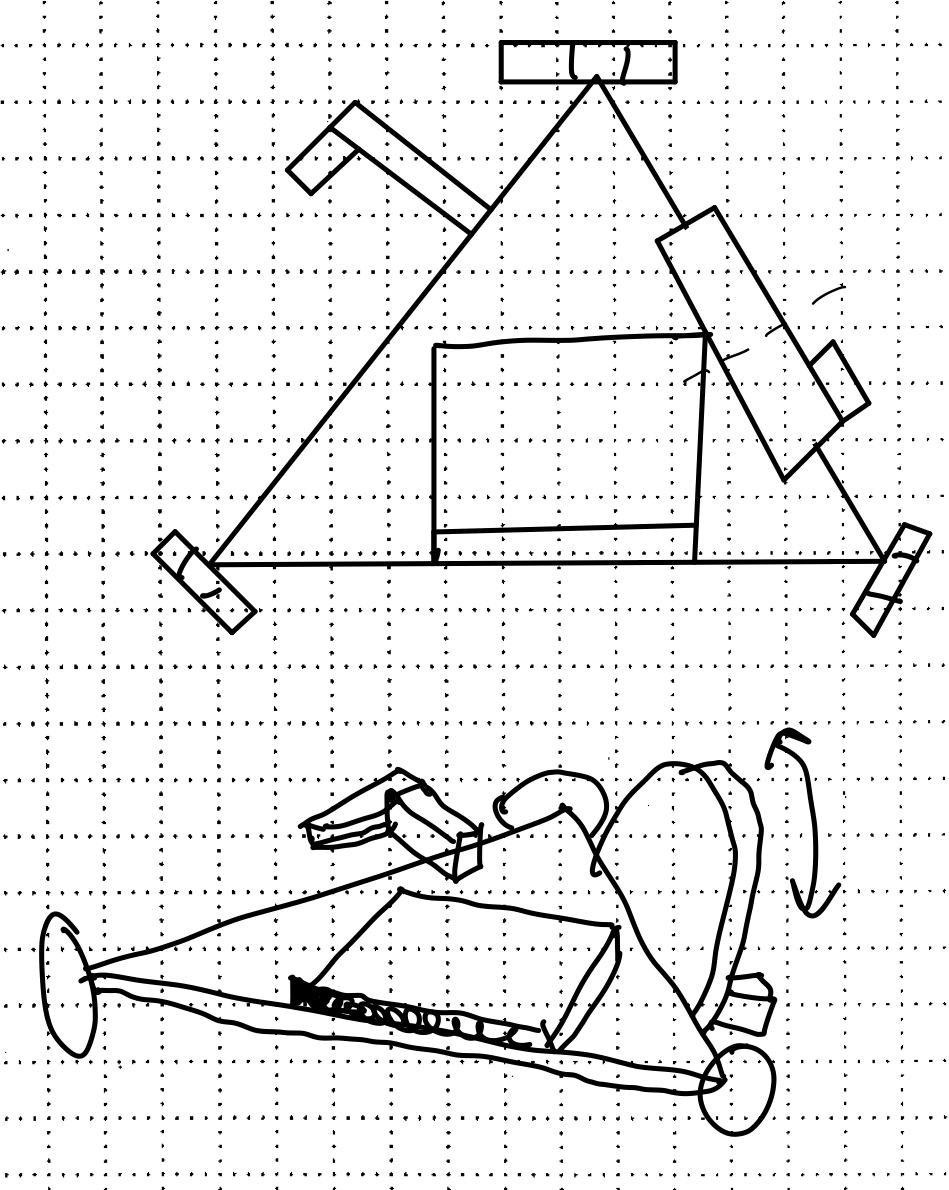
\includegraphics[width=0.6\textwidth]{Omni.png}
    \caption{\centering Rough sketch of a potential layout of Design 1. Arrows indicate some moving parts.}
    \label{fig:omni}
\end{figure}

\subsubsection*{Design 2}
\begin{enumerate}
    \item Chassis/Drivetrain: 2 Powered, 2 Unpowered, Rectangular Chassis
    \item Ice Cream Lever: Rotating circle
    \item Burger Flip: Rotating circle
    \item Jukebox: 2 Extending arms
    \item Order Ticket: Extending arm
    \item Trash Deposition: Rotating ramp
    \item Final Button: Extending arm
\end{enumerate}
\begin{figure}[H]
    \centering
    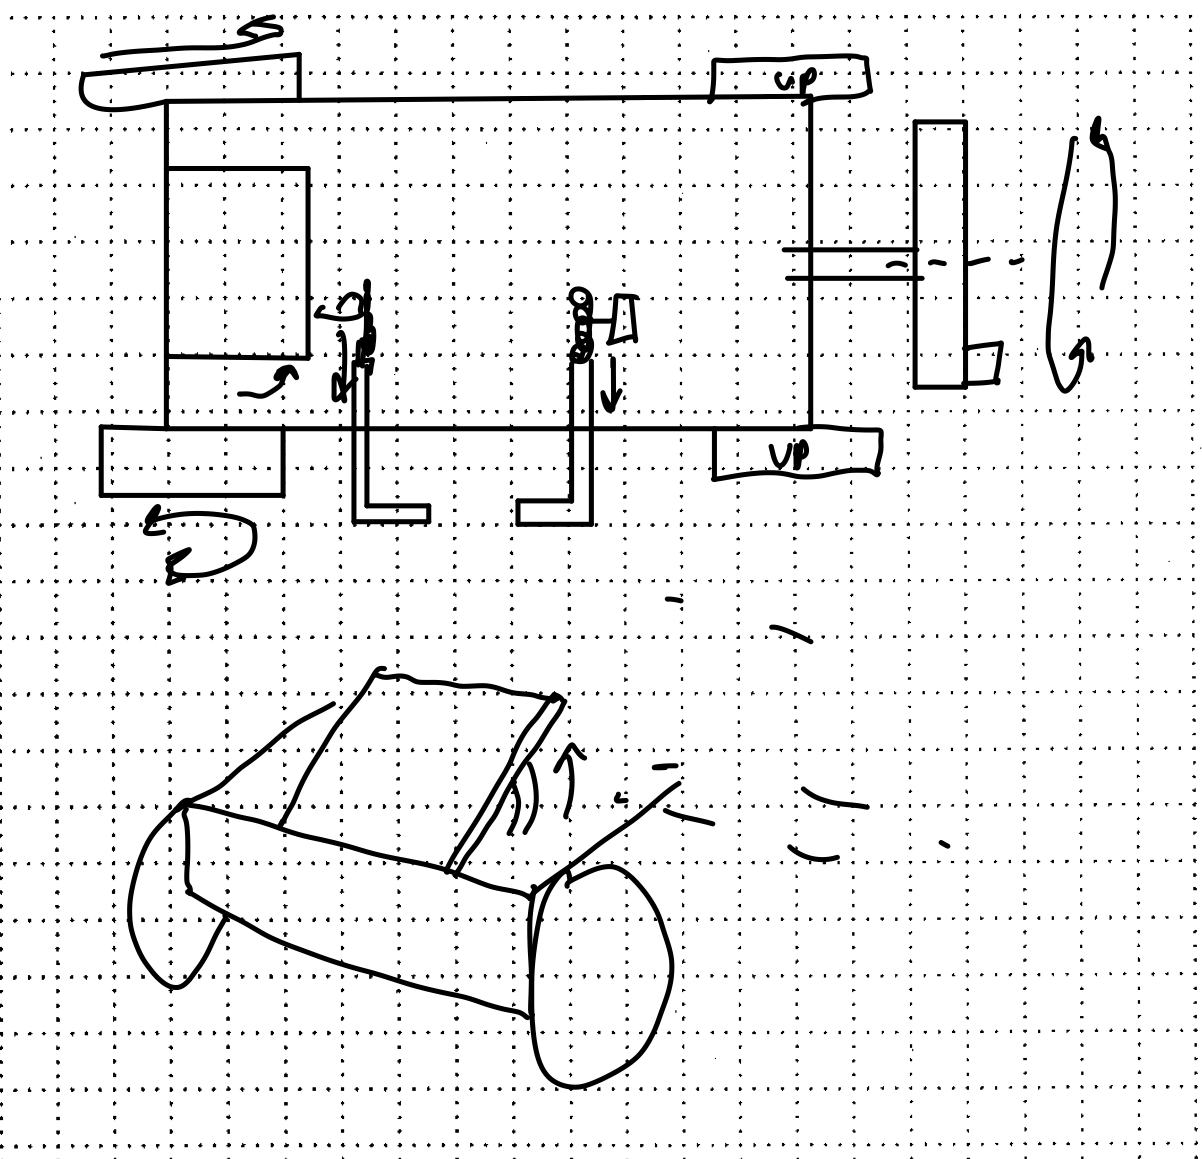
\includegraphics[width=0.6\textwidth]{Unpowered.png}
    \caption{\centering Rough sketch of a potential layout of Design 2. Arrows indicate some moving parts. "UP" indicates unpowered wheels.}
    \label{fig:unpowered}
\end{figure}

\subsubsection*{Design 3}
\begin{enumerate}
    \item Chassis/Drivetrain: 4 powered, Rectangular Chassis
    \item Ice Cream Lever: Rotating hook arm
    \item Burger Flip: Crane hook
    \item Jukebox: Extending arm
    \item Order Ticket: Extending arm
    \item Trash Deposition: Rotating ramp
    \item Final Button: Extending arm
\end{enumerate}
\begin{figure}[H]
    \centering
    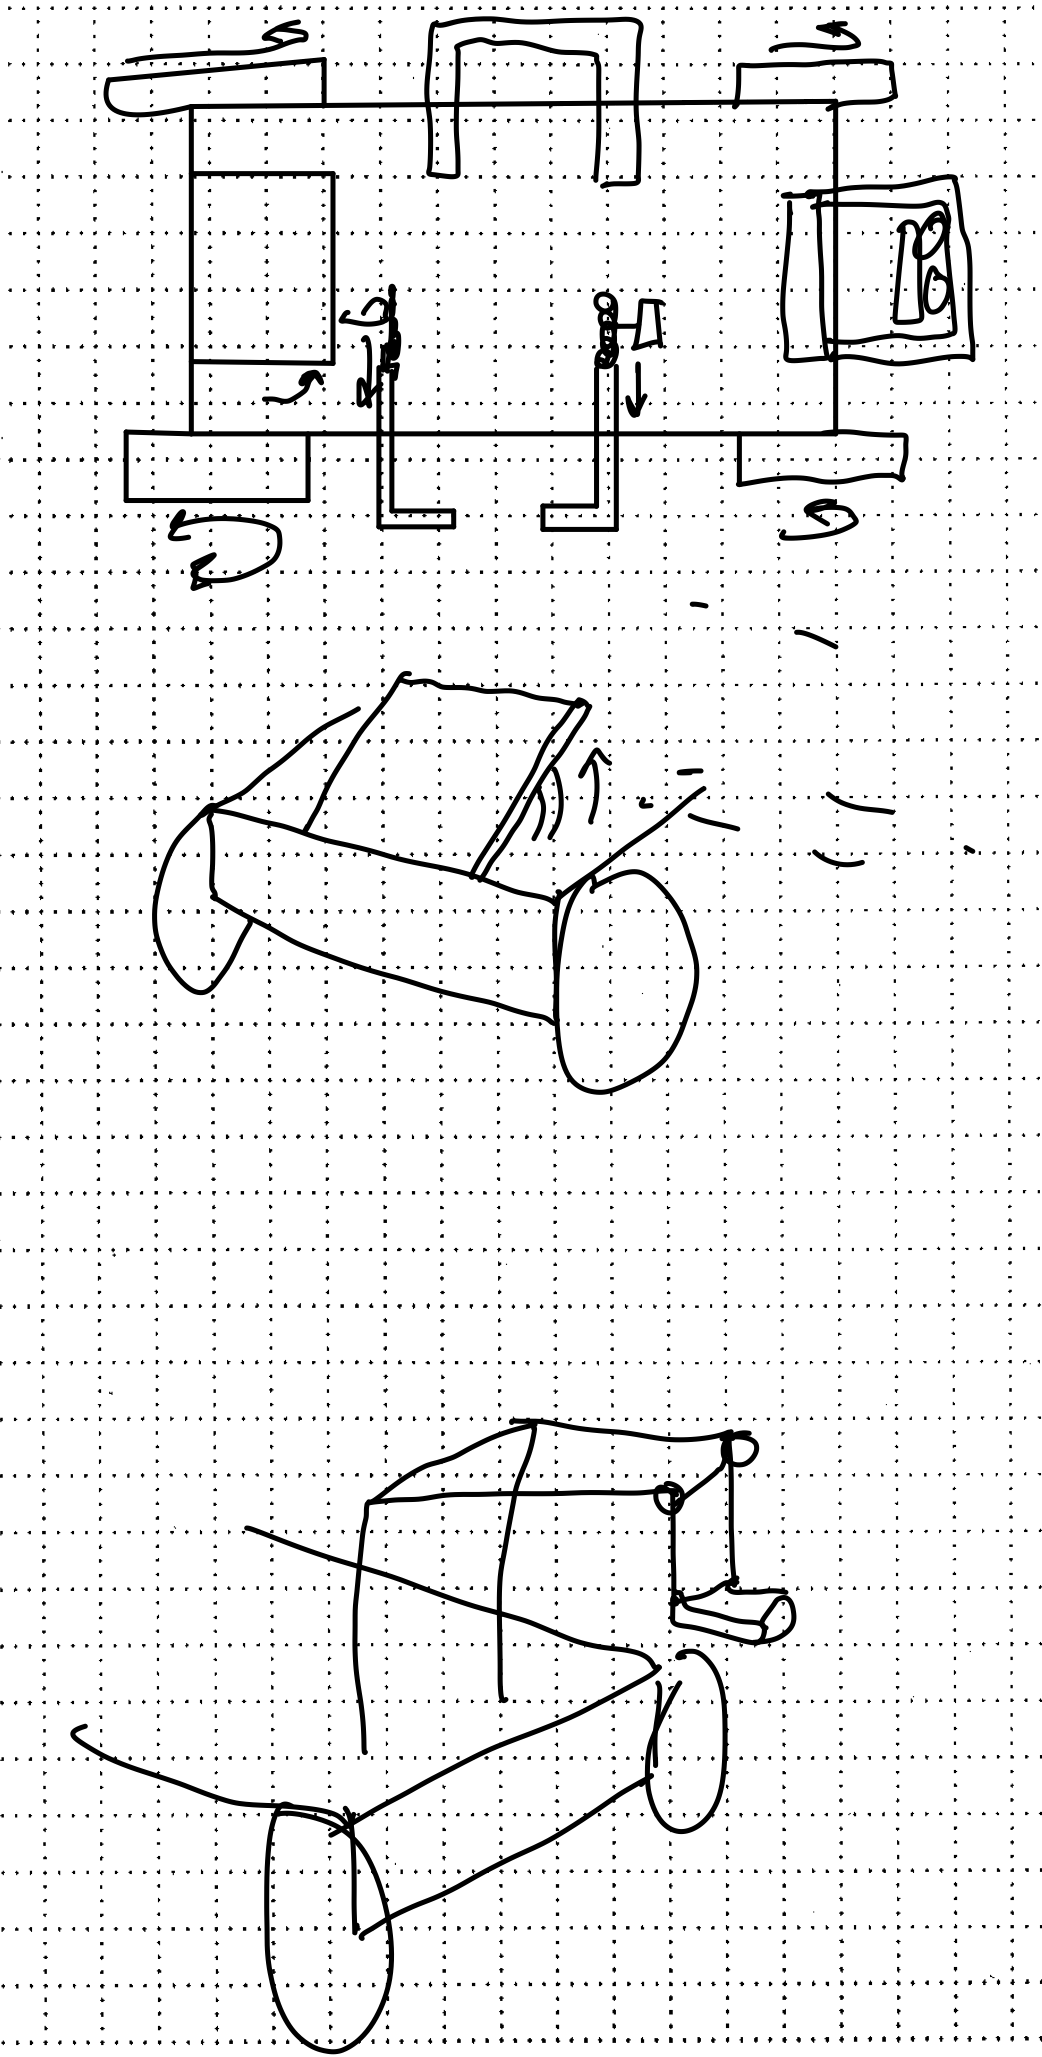
\includegraphics[width=0.6\textwidth]{fullpower.png}
    \caption{\centering Rough sketch of a potential layout of Design 3. Arrows indicate some moving parts.}
    \label{fig:fullpower}
\end{figure}

\subsection*{Ranking/Pros and Cons}
\subsubsection*{Rank 3: Design 3}
Pros:
\begin{enumerate}
    \item Moderate mobility and driving power is allowed by having four motors.
    \item The extending arms and ramp shouldn't require too fine of alignment to work and won't require much movement by the robot.
\end{enumerate}
Cons:
\begin{enumerate}
    \item Most expensive of the designs.
    \item Articulating the crane could prove difficult and introduce uncertainty as to location/sway.
\end{enumerate}

\subsubsection*{Rank 2: Design 2}
Pros:
\begin{enumerate}
    \item Uses the least amount of motors out of the designs.
    \item The extending arms and ramp shouldn't require too fine of alignment to work and won't require much movement by the robot.
\end{enumerate}
Cons:
\begin{enumerate}
    \item The robot will have a certain turn radius that it will have to look out for.
    \item Aligning the robot laterally is time consuming and difficult.
    \item The rotating circle will have to be dimensioned fairly precisely to allow it to function correctly.
\end{enumerate}

\subsubsection*{Rank 1: Design 1}
Pros:
\begin{enumerate}
    \item Full range of motion regardless of orientation.
    \item Allows position to be fine tuned quickly.
    \item Driving the nubs into specific spots should prove trivial.
    \item If the rotating circle is positioned and scaled correctly, it should allow the burger flip to be fairly trivial.
\end{enumerate}
Cons:
\begin{enumerate}
    \item Programming rotation and movement may be difficult.
    \item Programming aligning the robot to specific orientations could prove difficult.
    \item The rotating circle will have to be dimensioned fairly precisely to allow it to function correctly.
\end{enumerate}

\end{document}
